\chapter{Laplacians}
In future section the Gaussian random fields will be defined using the eigenvalues and eigenfunctions of the Dirichlet Laplacian. We will find that the Dirichlet Laplacian is an extension of the Kigami Laplacian. But to construct the Kigami Laplacian we will need the discrete Laplacian as we will prove that the Kigami Laplacian is the pointwise limit of the discrete Laplacian. We will therefore start by introducing first the discrete Laplacian, then the Kigami Laplacian and culminating in the Dirichlet Laplacian. Therefore consider the discrete Laplacian on the Vicsek set.
\begin{defi}\label{discreteLaplacian}
	Let $\ell(V_m)$ be the set of functions of $f: V_m \to \ree$. Then for any $f \in \ell(V_m)$  the \emph{discrete Laplacian} on $V_m$ is defined as
	\begin{equation}
		\Delta_m f(p) = 3^{m} \frac{1}{N_p}\sum_{q \in V_{m,p}} (f(q) - f(p)), \quad p \in V_m \backslash V_0
	\end{equation}
	where $$N_p = \begin{cases}
		5^{-m} & \text{if } \# V_{m,p} = 4 \\
		2\cd 5^{-(m+1)} & \text{if } \# V_{m,p} = 2\\
		5^{-(m+1)}  & \text{if } \# V_{m,p} = 1
	\end{cases}$$
\end{defi}

\begin{remark}\label{discreteMatrix}
	One is able to describe the discrete Laplacian as a matrix. First let $p_1, \ldots p_{N_m}$ be the vertices in $V_m$ then the \emph{Laplacian matrix} $L_m$ is constructed in the following way:
	\begin{equation}
		L_{i,j} = \begin{cases}
			\#V_{m,p_i}, & \text{if } i= j \\
			-1, & \text{if } i \neq j \text{ and } p_j \in V_{m,p_i} \\
			0, & \text{otherwise.}
		\end{cases}
	\end{equation}
Further $\#V_{m,p_i}$ is also called the \emph{degree of $p_i$}
\end{remark}

\section{Graph Energies}
In this section we will be following the arguments given by in chapter 1 of \cite{strichartz}. Many of the proof are going to rely on the graph energy. Thus we are first going to define and prove some properties of the graph eneriges form.

\begin{defi}
	Given a finite connected graph $G$ and it vertices $V_m$ the for functions $u, v: V_m \to \ree$ we define the \emph{graph energy} to be
	\begin{equation}\label{graphEnergy}
		E_m(u,v) = \sum_{x \sim y} \left(u(x) - u(y) \right)(v(x)-v(y)).
	\end{equation}
\end{defi}
\noindent \textbf{Notation:} We will write $E_m(u) = E_m(u,u)$.

 Since we in the end want to work on the whole of the Vicsek set $K$. We will want to create an extension of a function $u: V_m \to \ree$, such that it is defined on $V_{m+n}$. This is done in the following way

\begin{defi}
	Let $K$ be a graph and $u: V_m \to \ree$, then an \emph{extension of} $u$ is a function \nl $u': V_{m+n} \to \ree$ where $u' \mid_{V_m} = u$.
\end{defi}

It is obvious that $E_{m+n}(u') \geq E_m(u)$. Further one quickly notices that there must be a function that minimizes the graph Dirichlet form of a given graph. We denote such a function with $\tilde{u}$ and call it a \emph{harmonic extension}.

\begin{defi}
	Let $\tilde{u}: V_{m+n} \to \ree$ with $\title{u} \mid_{V_m} = u$ is called a \emph{harmonic extension} if $E_{m+n}(\tilde{u}) \leq E_{m+n}(u')$ for all $u': V_{m+n} \to \ree$ with $u' \mid _{V_m} = u$.
\end{defi}

 In some cases we have that $E_{m+n}(\tilde{u}) = r^{n} E_{m}(u)$ for some $r \in (0,1)$. But instead of normalizing the values on $E_m$ we will normalize $E_{m+n}$. Thus  getting
\begin{equation}
	r^{-n} E_{m+n}(\tilde{u}) = E_m(u), \quad \text{and} \quad r^{-n} E_{m+n}(u') \geq E_m(u)
\end{equation}
for every extension $u'$ of $u$. The constant $r$ is called the \emph{renormalization constant} From the equality above we can define the following
\begin{defi}\label{renormalizedGraphEnergies}
	The \emph{renormalized graph energy} are defined as
	\begin{equation}
		\eee_{m}(u) = r^{-m}E_m(u)
	\end{equation}
	Note that the sequence $\cbr{\eee_{m}(u)}$ is a non-decreasing sequence. 
\end{defi}

Based on this definition we see that for a harmonic extension $\tilde{u}$ of $u$ we have that 
\begin{equation}
	\mathcal{E}_{m+1}(\tilde{u}) = r^{-(m+1)}E_{m+1}(\tilde{u}) = r^{-m}E_{m}(u) = \mathcal{E}_{m}(u).
\end{equation}
Extending this to the bilinear form we have for harmonic extension $\tilde{u}, \tilde{v}$ of $u, v$ that
\begin{equation}
	\mathcal{E}_{m+1}(\tilde{u}, \tilde{v}) = \mathcal{E}_{m}(u,v).
\end{equation}

Actually one even has that for the bilinear form then if $\tilde{u}$ is the harmonic extension of $u$ and $v'$ is any extension of $v$ then
\begin{equation}\label{bilinearFormRenormalized}
	\mathcal{E}_{m+1}(\tilde{u}, v') = \mathcal{E}_{m}(u,v).
\end{equation}
See \cite{strichartz} for further details.

Now that we have \cref{renormalizedGraphEnergies}, we can define what it means to be a harmonic function.


\begin{defi}
	$u$ is a \emph{harmonic function} if $u$ minimizes $\eee_{m}(u)$ for all $m$, given boundary values on $V_0$.
\end{defi}

The harmonic functions will be used extensively throughout this section. We start by finding the renormalization constant for the Vicsek set.

\subsection{Renormalization constant on the Vicsek set}

I the previous section we have talked about a harmonic function, but without every constructing one. We will therefore in this next section show how to create an harmonic function for the Vicsek set for any start boundary values.

Given $V_0 = \cbr{q_0, q_1, q_2, q_3, q_4}$ and $u: V_0 \to \ree$ then we have that
\begin{equation}
	E_0(u) = \left(u(q_0) - u(q_1)\right)^2 + \left(u(q_0) - u(q_2)\right)^2 + \left(u(q_0) - u(q_3)\right)^2 + \left(u(q_0) - u(q_4)\right)^2.
\end{equation} 
We are going to exploit symmetry of the Vicsek set. Since all four "limbs" of the Vicsek set are identical we will only look at one of the limbs since the other limbs will be the same computations. So if we want to minimize $E_1(u')$, we see for the limb between $q_0$ and $q_1$ that
\begin{multline}
	E_1(u') = \left(u'(q_1) - u'(p_0)\right)^2 + \left(u'(p_0) - u'(p_2)\right)^2 \\
	 + \left(u'(p_0) - u'(p_3)\right)^2 + \left(u'(p_0) - u'(p_4)\right)^2 + \left(u'(p_3) - u'(q_0)\right)^2.
\end{multline}


\begin{figure}[!ht] \label{renormVicsekDiagram}
	\centering
	\tikzset{every picture/.style={line width=0.75pt}} %set default line width to 0.75pt        
	
	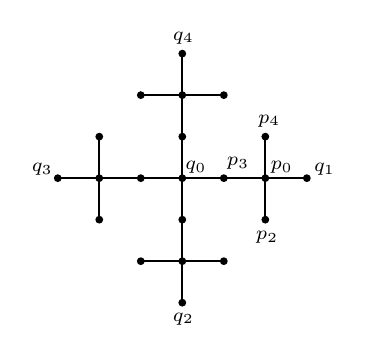
\begin{tikzpicture}[x=0.75pt,y=0.75pt,yscale=-1,xscale=1]
		%uncomment if require: \path (0,300); %set diagram left start at 0, and has height of 300
		
		%Straight Lines [id:da6304295946642043] 
		\draw    (200,120) -- (200,240) ;
		\draw [shift={(200,240)}, rotate = 90] [color={rgb, 255:red, 0; green, 0; blue, 0 }  ][fill={rgb, 255:red, 0; green, 0; blue, 0 }  ][line width=0.75]      (0, 0) circle [x radius= 1.34, y radius= 1.34]   ;
		\draw [shift={(200,120)}, rotate = 90] [color={rgb, 255:red, 0; green, 0; blue, 0 }  ][fill={rgb, 255:red, 0; green, 0; blue, 0 }  ][line width=0.75]      (0, 0) circle [x radius= 1.34, y radius= 1.34]   ;
		%Straight Lines [id:da15009868113581337] 
		\draw [color={rgb, 255:red, 0; green, 0; blue, 0 }  ,draw opacity=1 ]   (140,180) -- (260,180) ;
		\draw [shift={(260,180)}, rotate = 0] [color={rgb, 255:red, 0; green, 0; blue, 0 }  ,draw opacity=1 ][fill={rgb, 255:red, 0; green, 0; blue, 0 }  ,fill opacity=1 ][line width=0.75]      (0, 0) circle [x radius= 1.34, y radius= 1.34]   ;
		\draw [shift={(140,180)}, rotate = 0] [color={rgb, 255:red, 0; green, 0; blue, 0 }  ,draw opacity=1 ][fill={rgb, 255:red, 0; green, 0; blue, 0 }  ,fill opacity=1 ][line width=0.75]      (0, 0) circle [x radius= 1.34, y radius= 1.34]   ;
		%Straight Lines [id:da6360387946571586] 
		\draw    (160,160) -- (160,200) ;
		\draw [shift={(160,200)}, rotate = 90] [color={rgb, 255:red, 0; green, 0; blue, 0 }  ][fill={rgb, 255:red, 0; green, 0; blue, 0 }  ][line width=0.75]      (0, 0) circle [x radius= 1.34, y radius= 1.34]   ;
		\draw [shift={(160,160)}, rotate = 90] [color={rgb, 255:red, 0; green, 0; blue, 0 }  ][fill={rgb, 255:red, 0; green, 0; blue, 0 }  ][line width=0.75]      (0, 0) circle [x radius= 1.34, y radius= 1.34]   ;
		%Straight Lines [id:da967738390323848] 
		\draw    (240,160) -- (240,200) ;
		\draw [shift={(240,200)}, rotate = 90] [color={rgb, 255:red, 0; green, 0; blue, 0 }  ][fill={rgb, 255:red, 0; green, 0; blue, 0 }  ][line width=0.75]      (0, 0) circle [x radius= 1.34, y radius= 1.34]   ;
		\draw [shift={(240,160)}, rotate = 90] [color={rgb, 255:red, 0; green, 0; blue, 0 }  ][fill={rgb, 255:red, 0; green, 0; blue, 0 }  ][line width=0.75]      (0, 0) circle [x radius= 1.34, y radius= 1.34]   ;
		%Straight Lines [id:da22729733453474055] 
		\draw    (220,140) -- (180,140) ;
		\draw [shift={(180,140)}, rotate = 180] [color={rgb, 255:red, 0; green, 0; blue, 0 }  ][fill={rgb, 255:red, 0; green, 0; blue, 0 }  ][line width=0.75]      (0, 0) circle [x radius= 1.34, y radius= 1.34]   ;
		\draw [shift={(220,140)}, rotate = 180] [color={rgb, 255:red, 0; green, 0; blue, 0 }  ][fill={rgb, 255:red, 0; green, 0; blue, 0 }  ][line width=0.75]      (0, 0) circle [x radius= 1.34, y radius= 1.34]   ;
		%Straight Lines [id:da18095273720450344] 
		\draw    (170,180) -- (185.5,180) -- (190,180) ;
		%Straight Lines [id:da24264648223015173] 
		\draw    (220,220) -- (180,220) ;
		\draw [shift={(180,220)}, rotate = 180] [color={rgb, 255:red, 0; green, 0; blue, 0 }  ][fill={rgb, 255:red, 0; green, 0; blue, 0 }  ][line width=0.75]      (0, 0) circle [x radius= 1.34, y radius= 1.34]   ;
		\draw [shift={(220,220)}, rotate = 180] [color={rgb, 255:red, 0; green, 0; blue, 0 }  ][fill={rgb, 255:red, 0; green, 0; blue, 0 }  ][line width=0.75]      (0, 0) circle [x radius= 1.34, y radius= 1.34]   ;
		%Straight Lines [id:da6311736325856517] 
		\draw    (180,180) -- (160,180) ;
		\draw [shift={(160,180)}, rotate = 180] [color={rgb, 255:red, 0; green, 0; blue, 0 }  ][fill={rgb, 255:red, 0; green, 0; blue, 0 }  ][line width=0.75]      (0, 0) circle [x radius= 1.34, y radius= 1.34]   ;
		\draw [shift={(180,180)}, rotate = 180] [color={rgb, 255:red, 0; green, 0; blue, 0 }  ][fill={rgb, 255:red, 0; green, 0; blue, 0 }  ][line width=0.75]      (0, 0) circle [x radius= 1.34, y radius= 1.34]   ;
		%Straight Lines [id:da868237351757014] 
		\draw    (240,180) -- (220,180) ;
		\draw [shift={(220,180)}, rotate = 180] [color={rgb, 255:red, 0; green, 0; blue, 0 }  ][fill={rgb, 255:red, 0; green, 0; blue, 0 }  ][line width=0.75]      (0, 0) circle [x radius= 1.34, y radius= 1.34]   ;
		\draw [shift={(240,180)}, rotate = 180] [color={rgb, 255:red, 0; green, 0; blue, 0 }  ][fill={rgb, 255:red, 0; green, 0; blue, 0 }  ][line width=0.75]      (0, 0) circle [x radius= 1.34, y radius= 1.34]   ;
		%Straight Lines [id:da7980791265955824] 
		\draw    (200,220) -- (200,200) ;
		\draw [shift={(200,200)}, rotate = 270] [color={rgb, 255:red, 0; green, 0; blue, 0 }  ][fill={rgb, 255:red, 0; green, 0; blue, 0 }  ][line width=0.75]      (0, 0) circle [x radius= 1.34, y radius= 1.34]   ;
		\draw [shift={(200,220)}, rotate = 270] [color={rgb, 255:red, 0; green, 0; blue, 0 }  ][fill={rgb, 255:red, 0; green, 0; blue, 0 }  ][line width=0.75]      (0, 0) circle [x radius= 1.34, y radius= 1.34]   ;
		%Straight Lines [id:da7384137154814034] 
		\draw    (200,160) -- (200,140) ;
		\draw [shift={(200,140)}, rotate = 270] [color={rgb, 255:red, 0; green, 0; blue, 0 }  ][fill={rgb, 255:red, 0; green, 0; blue, 0 }  ][line width=0.75]      (0, 0) circle [x radius= 1.34, y radius= 1.34]   ;
		\draw [shift={(200,160)}, rotate = 270] [color={rgb, 255:red, 0; green, 0; blue, 0 }  ][fill={rgb, 255:red, 0; green, 0; blue, 0 }  ][line width=0.75]      (0, 0) circle [x radius= 1.34, y radius= 1.34]   ;
		%Straight Lines [id:da3701955076323855] 
		\draw    (200,200) -- (200,180) ;
		\draw [shift={(200,180)}, rotate = 270] [color={rgb, 255:red, 0; green, 0; blue, 0 }  ][fill={rgb, 255:red, 0; green, 0; blue, 0 }  ][line width=0.75]      (0, 0) circle [x radius= 1.34, y radius= 1.34]   ;
		
		% Text Node
		\draw (200,170.4) node [anchor=north west][inner sep=0.75pt]  [font=\scriptsize]  {$q_{0}$};
		% Text Node
		\draw (262,171.4) node [anchor=north west][inner sep=0.75pt]  [font=\scriptsize]  {$q_{1}$};
		% Text Node
		\draw (194,108) node [anchor=north west][inner sep=0.75pt]  [font=\scriptsize]  {$q_{4}$};
		% Text Node
		\draw (194,243.4) node [anchor=north west][inner sep=0.75pt]  [font=\scriptsize]  {$q_{2}$};
		% Text Node
		\draw (126,171.4) node [anchor=north west][inner sep=0.75pt]  [font=\scriptsize]  {$q_{3}$};
		% Text Node
		\draw (241,170.4) node [anchor=north west][inner sep=0.75pt]  [font=\scriptsize]  {$p_{0}$};
		% Text Node
		\draw (220,168.4) node [anchor=north west][inner sep=0.75pt]  [font=\scriptsize]  {$p_{3}$};
		% Text Node
		\draw (234,204) node [anchor=north west][inner sep=0.75pt]  [font=\scriptsize]  {$p_{2}$};
		% Text Node
		\draw (235,148) node [anchor=north west][inner sep=0.75pt]  [font=\scriptsize]  {$p_{4}$};
				
	\end{tikzpicture}
	\caption{Points on the Vicsek set}
\end{figure}
We are then going to optimize with regards to $u'(p_i)$ for $i = 0, 1, 2, 4$. Taking the derivative of the right side and solving for $0$ we get the following
\begin{align}
	4 u'(p_0) &= u'(q_1) + u'(p_2) + u'(p_3) + u'(p_4) \\
	2 u'(p_3) &= u'(q_0) + u'(p_0) \\
	u'(p_2) &= u'(p_0)\\
	u'(p_4) &= u'(p_0).
\end{align}
Solving these equations we get
\begin{align}
	u'(p_0) &=  \frac{2}{3} u'(q_1) + \frac{1}{3} u'(q_0)\\
	u'(p_2) &= \frac{2}{3} u'(q_1) + \frac{1}{3} u'(q_0) \\
	u'(p_4) &= \frac{2}{3} u'(q_1) + \frac{1}{3} u'(q_0) \\
	u'(p_3) &= \frac{2}{3} u'(q_0) + \frac{1}{3} u'(q_1).
\end{align}

So what we have found is that to minimize the value in the points of the Vicsek set, then the value in the next point is going to be $2/3$ the value from the closest point and $1/3$ the value from the next closest point. 

If one calculates the graph energy they will find
\begin{equation}
	E_1(u') =\frac{1}{3}\sum_{i = 1}^{4}(u'(q_i) - u'(q_0))^2 = \frac{1}{3}E_0(u').
\end{equation}

Since the Vicsek set is a self-similar set, we have that going from $V_1$ to $V_2$ is the same as going from $V_m$ to $V_{m+1}$. Thus we can just extend the above calculations to doing it $m$ times, in which case
\begin{equation}
	E_{m+1}(u') = \frac{1}{3}E_m(u')
\end{equation}

Thus we get our renormalization constant for the vicsek set to be $r = \frac{1}{3}$. And altogether we find that from \cref{renormalizedGraphEnergies} we have that 
\begin{equation}
	\mathcal{E}_{m}(u) = 3^{m} E_{m}(u).
\end{equation}


\section{Kigami Laplacian}
With the renormalization constant found we will return to finding the Kigmai Laplacian. Recall from \cref{renormalizedGraphEnergies} that we have defined a sequence $\mathcal{E}_m$ for functions on $V^{*}$. It will therefore make sense to define the following limit
\begin{defi}\label{renormalizedGraphEnergiesLimit} Let $u: V^{*} \to \ree$ then define the limit
	\begin{equation}
		\mathcal{E}(u, u) = \lim_{m \to \infty} \mathcal{E}_{m}(u, u)
	\end{equation}
	where we set
	\begin{equation}
		\dom \mathcal{E} = \cbr{u \in \ell(V_{*}) : \mathcal{E}(u) < \infty}.
	\end{equation}
	and denote $\dom_0 \mathcal{E}$ with the functions in $\dom \mathcal{E}$ that vanish $V_0$.
\end{defi}

This definition only involves functions defined on $V^{*}$, but we find that functions in $\dom \mathcal{E}$ are uniformly continuos and therefore has an unique extension to $K$. We even have that $\dom \mathcal{E}$ is dense in $C(K)$.
\begin{prop} \phantom{a}
	\begin{enumerate}[(i)] 
		\item 	Let $u \in \dom \mathcal{E}$ then $u$ is uniformly continuous on $V^{*}$. \label{uniCont1}
		\item $\dom \mathcal{E}$ is dense in $C(K)$. \label{uniCont2}
	\end{enumerate}
\end{prop}
\begin{proof}
	We start with (\ref{uniCont1}). Let $u \in \dom \mathcal{E}$ then $\mathcal{E}_m(u) \leq \mathcal{E}(u)$ since $\mathcal{E}_m$ is non-decreasing in $m$. So for $x,y \in V_m$ if $y \in V_{m,x}$we have that
	\begin{equation}\label{uniFormContiousEstimate}
		r^{-m}(u(x) -u(y))^{2} \leq \mathcal{E}_m(u) \leq \mathcal{E}(u)
	\end{equation}
	since $r^{-m}(u(x) -u(y))^{2}$ is a term in $\mathcal{E}_m(u)$. Thus
	\begin{equation}
		\abs{u(x)-u(y)} \leq r^{\frac{m}{2}} \mathcal{E}(u)^{\frac{1}{2}}.
	\end{equation}
	
	\textcolor{red}{I cannot get this to be uniformly convergent.}
	Now consider a chain of points $x_m, x_{m+1}, \ldots, x_{m+k}$ where $x_{m+j} \in V_{m+j}$ and $x_{m+j} \in V_{m+j+1, x_{m+j+1}}$. Then we have
	\begin{equation}
		\abs{u(x_m)-u(x_{m+k})} \leq r^{\frac{m}{2}}\left(1 + r^{\frac{1}{2}} + \ldots + r^{\frac{k}{2}}\right)\mathcal{E}(u)^{\frac{1}{2}} \leq \frac{r^{m}}{1-r^{\frac{1}{2}}} \mathcal{E}^{\frac{1}{2}}
	\end{equation}
	by using \eqref{uniFormContiousEstimate} and the triangle inequality multiple times. From the geometry of $K$ we see that $x, y \in V^{*}$ belong to the same or adjacent $m$-cells then we can connect $x$ to $y$ by at most $2$ such chains \textcolor{red}{What does he mean?}, so
	\begin{equation}
		\abs{u(x) - u(y)} \leq \frac{2r^{m/2}}{1-r^{\frac{1}{2}}} \mathcal{E}(u)^{\frac{1}{2}}
	\end{equation}
	and we have a bound for all $x,y \in V^{*}$.
	
	For proof of (\ref{uniCont2}) we refer to \cite{strichartz}.
\end{proof}


We are now ready to define the Kigami Laplacian. We will denote this with $\Delta_{\mu}$ and we will notice that it depends on a measure $\mu$, which will be the one defined in \eqref{normalziedHausdorffMeasure}.
\begin{defi}
	Let $u \in \dom \mathcal{E}$ and let $f$ be continuos, then $u \in \dom \Delta_{\mu}$ and $\Delta_{\mu} u =f$ if
	\begin{equation}
		\mathcal{E}(u,v) = \int_{K}fv \dd \mu, \quad \forall v \in \dom_{0}\mathcal{E}
	\end{equation}
\end{defi}

As mentioned before  we are going to want $\Delta_{\mu}$ to be defined as the limit of $\Delta_m$. The constants $3^m$ and $5^m$ are not random, but chosen such that the Kigami Laplacian makes sense. But to prove the pointwise limit and actually calculate the constants, we will need a few lemmas and definitions. Since we will be finding the constant we introduce a new notation for the discrete graph Laplacian without its constants. We start by defining this graph Laplacian and then followed by a harmonic function which will be used extensively in the following proofs.

\begin{defi}
	Let $\Delta_{m}$ be defined as in \cref{discreteLaplacian}, we then define
	\begin{equation}
		\widetilde{\Delta}_{m}f(p) = 3^{-m} N_p \Delta_mf(p).
	\end{equation}
\end{defi}

\begin{defi}
	Given $m$ and a point $x \in V_m \backslash V_0$ then define the harmonic function $\psi_{x}^{m}: V^{*} \to [0,1]$ that for a $y \in V_m$ is $\psi_x^{(m)}(y) = \delta_{xy}$.
\end{defi}
I might seem that we have only defined $\psi_x^{(m)}$ to have values on $V_m$. But the function is defined on the whole of $V^{*}$, where the values in $K \backslash V_m$ comes from the fact that it is an harmonic extension. We even have that function $\psi_x^{(m)}$ can be used to describe $\widetilde{\Delta}_{m}$.
\begin{prop}\label{pointwiseEqualityofpsi}
	Let $u \in \dom \mathcal{E}$ and $\Delta_{\mu}u = f$then
	\begin{equation}
		r^{-m}\widetilde{\Delta}_{m}u(x) = \int_{K}f \psi_{x}^{(m)} \dd \mu
	\end{equation}
\end{prop}
\begin{proof}
	We see that
	\begin{equation}
		\mathcal{E}_{m}(u, \psi_{x}^{(m)}) = r^{-m} \sum_{p \underset{m}{\sim} q}(u(q)-u(p))(\psi_{x}^{(m)}(p) -\psi_{x}^{(m)}(q)) = r^{-m}\sum_{q \in V_{m,x}}(u(x)-u(q)) = r^{-m}\widetilde{\Delta}_{m}u(x)
	\end{equation}
	where the second equality comes the fact that only edges containing $x$ are going to see change in $\psi_{x}^{(m)}$. Now by \eqref{bilinearFormRenormalized} we have that
	\begin{equation}
		r^{-m}\widetilde{\Delta}_{m}u(x) = \mathcal{E}_{m}(u, \psi_{x}^{(m)}) = \mathcal{E}(u, \psi_{x}^{(m)}) = \int_{K}f \psi_{x}^{(m)} \dd \mu
	\end{equation}
	as desired.
\end{proof}

\begin{lemma}\label{itIsZero}
	Let $v: V^{*} \to \ree$ be a harmonic function on the Vicsek set. If $v(x) = v(y_i) = 0$ for all $y_i \in V_{m,x}$ then $v(\omega) = 0$ for all $\omega \in \overline{B_x}$ where $B_x = \left( \bigcup_{k > 0} S^{k}(x) \right) \cup \left(\bigcup_{i} \{y_i\} \right)$
\end{lemma}
\begin{proof}
	It is clear that $v(\omega) = 0$ for any $\omega \in B_x$, since the value of the points $S^{k}(x)$ with $k > 0$ depends on the value of $x$ and its neighbours. 
	
	So we need to check the points in $\overline{B_x} \backslash B_x$. Now since $B_x$ is dense in $\overline{B_x}$, then for any $\omega \in \overline{B_x}$ we have that there exists a sequence $x_n \in B_x$ such that $x_n \to \omega$. By the fact that $v$ is continuos on $K$ it is continuos on $\overline{B_x}$, in which case $\abs{v(x_n) - v(\omega)} \to 0$ as $n \to \infty$, but $v(x_n) = 0$ for all $x_n$, so $v(\omega) = 0$ as desired.  
\end{proof}

What lemma $\ref{itIsZero}$ sates, is if any two points in $V_m$ are neighbours, say $x$ and $y$, and $v(x)=v(y)=0$, then then function value at any point between $x$ and $y$ is also zero.

\begin{lemma}\label{FmSmaller}
	Set $F_m = \supp \psi_{x}^{(m)}$, then
	\begin{equation}
		F_0 \supset F_1 \supset F_2 \supset F_3 \supset \dots
	\end{equation}
	Further $F_m$ is contained in the open ball $B(x, \epsilon_m)$ where $\epsilon_m \to 0$ as $m \to \infty$.
\end{lemma}

\begin{proof}
	If we set $\Omega_m = \left\{z \in K : \psi_{x}^{(m)}(z) = \psi_{x}^{(m)}(y) = 0, \forall y \in V_{m,z}  \right\}$ then $F_m = K \backslash \left(\bigcup_{\alpha \in \Omega_m} \overline{B_\alpha} \right)$. It is clear that $\Omega_m \subset \Omega_{m+1}$ and that there are new points in $\Omega_{m+1}$ that are not just a point between some already existing points $x_1, x_2 \in \Omega_m$. We therefore have from the way that $F_m$ is constructed that $F_m \supset F_{m+1}$.
	
	The containment of $F_m$ in $B(x, \epsilon_m)$ follows from \cref{itIsZero} and that $F_m \supset F_{m+1}$.
\end{proof}

We are now ready to prove the pointwise formula

\begin{theorem} \label{pointwiseFormula}
	Let $u \in \dom \Delta_{\mu}$. Then the pointwise formula
	\begin{equation}
		\Delta_{\mu} u(x) = \lim_{m \to \infty} r^{-m} \left(\int_{K} \psi_x^{(m)} \dd \mu \right)^{-1} \widetilde{\Delta}_m u(x)
	\end{equation}
	holds with the limit uniform across $V_* \backslash V_0$. Conversely, suppose $u$ is a continuos function and the right side of the limit converges uniformly to a continuos function on $V_* \backslash V_0$. Then $u \in \dom \Delta_{\mu}$ and the equation holds.
\end{theorem}

\begin{proof}
	Suppose $u \in \dom \Delta_{\mu}$ and $\Delta_{\mu} u=f$, then by \cref{pointwiseEqualityofpsi} we have that 
	\begin{equation}
		r^{-m} \left(\int_{K} \psi^{(m)}_{x} \dd\mu \right)^{-1} \widetilde{\Delta}_m u(x) = \frac{\int_{K} f \psi_x^{(m)} \dd\mu}{\int_{K} \psi_x^{(m)} \dd\mu}
	\end{equation}
	for any $x \in V_m \backslash V_0$. The right side needs to converge uniformly, so let $\epsilon > 0$. Since $f(x)$ is continuos then by \cref{FmSmaller} we can choose $m$ large enough so for all $x, y \in F_m$ that $\abs{f(x) - f(y)} < \epsilon$, then
	\begin{align}
		\abs{\frac{\int_{K} f \psi_x^{(m)} \dd\mu}{\int_{K} \psi_x^{(m)} \dd\mu} - f(x)} &= \abs{\frac{\int_{K} f \psi_x^{(m)} \dd\mu}{\int_{K} \psi_x^{(m)} \dd\mu} - \frac{\int_{K} f(x) \psi_x^{(m)} \dd\mu}{\int_{K} \psi_x^{(m)} \dd\mu}} \\
		&= \abs{\frac{\int_{K} \left(f(y) -f(x) \right) \psi_x^{(m)} \dd\mu}{\int_{K} \psi_x^{(m)} \dd\mu}} \\
		&\leq \frac{\int_{F_m} \abs{f(y) -f(x)} \dd\mu}{\int_{K} \psi_x^{(m)} \dd\mu} \\
		&\leq \frac{\epsilon \int_{F_m} \dd\mu}{\int_{K} \psi_x^{(m)} \dd\mu} \\
		&= \epsilon
	\end{align}
	in which case
	\begin{equation}
		\lim_{m \to \infty} r^{-m} \left(\int_{K} \psi^{(m)}_{x} \dd\mu \right)^{-1} \widetilde{\Delta}_m u(x) = \lim_{m \to \infty} \frac{\int_{K} f \psi_x^{(m)} \dd \mu}{\int_{K} \psi_x^{(m)} \dd \mu} = f(x) = \Delta_{\mu} u(x)
	\end{equation}
	
	
	Moving on to the second half of the proof. Suppose that $r^{m} \left(\int_{K} \psi_x^{(m)} \dd \mu \right)^{-1} \widetilde{\Delta}_m u(x)$ converges uniformly to a continuos function $f$. Now for any $v \in \dom_0 \mathcal{E}$ we have 
	\begin{equation}
		\mathcal{E}_m(u,v) = r^{-m} \sum_{x \underset{m}{\sim} y} \left( u(y) - u(x) \right)\left(v(y) - v(x) \right).
	\end{equation}
	
	If we collect all the terms that contain the factor $v(x)$ for a fixed $x \in V_m \backslash V_0$ then each $v(x)$ will be of the form $-v(x) \left(u(y) - u(x) \right)$ for each $y \underset{m}{\sim} x$. In which case we get
	\begin{align}
		\mathcal{E}_m(u,v) &= - r^{-m}  \sum_{x \in V_m \backslash v_0} v(x) \left( \sum_{x \underset{m}{\sim} y} \left( u(y) - u(x) \right) \right) \\
		&= -\sum_{x \in V_m \backslash V_0} v(x) r^{-m} \widetilde{\Delta}_{m}u(x)
	\end{align}
	While it seems we lose many terms by removing $v(y)$, but they are instead contained in 
	$$\sum_{x \underset{m}{\sim} y} \left( u(y) - u(x) \right).$$ 
	Note that the sum is "reset" for every $x$ so we count both the relation $x \sim y$ and $y \sim x$.
	
	Now if we define $f_m(x) = r^{-m} \left(\int_{K} \psi_{x}^{(m)} \dd\mu \right)^{-1} \widetilde{\Delta}_{m}u(x)$ then $f_m \to f$ uniformly by assumption and we can rewrite the above as   
	\begin{align}
		\mathcal{E}_m(u,v) &= -\sum_{x \in V_m \backslash V_0} v(x) \left(\int_{K} \psi_{x}^{(m)} \dd\mu \right) r^{-m} \left(\int_{K} \psi_{x}^{(m)} \dd\mu \right)^{-1} \widetilde{\Delta}_{m}u(x) \\
		&= - \int_{K} \left( \sum_{x \in V_m \backslash V_0} v(x) f_m(x) \psi_x^{(m)}\right) \dd \mu. \\
	\end{align}
	Since the convergence in the next calculation follows from a quite lengthy argument, we will show the calculation and then return to the convergence. So we have that 
	\begin{equation}\label{theVeryLongOne}
		\mathcal{E}(u, v) = \lim_{m \to \infty} \mathcal{E}_m(u,v) = \lim_{m \to \infty}-\int_{K} \left( \sum_{x \in V_m \backslash V_0} v(x) f_m(x) \psi_x^{(m)}\right) \dd \mu = - \int_{K} v(y)f(y) \dd \mu.
	\end{equation}
	and we have that $u \in \text{dom}\Delta_{\mu}$. Now looking at the convergence in \eqref{theVeryLongOne} we have
	\begin{multline}
		\abs{\sum_{x \in V_m \backslash V_0} v(x) f_m(x) \psi_x^{(m)}(y) -v(y)f(y)} \\
		\leq \abs{\sum_{x \in V_m \backslash V_0} \left(v(x) f_m(x) - v(y)f(y) \right) \psi_x^{(m)}(y)} + \abs{\sum_{x \in V_m \backslash V_0} v(y) f(y) \psi_x^{(m)}(y) -v(y)f(y)}
	\end{multline}
	Looking at each term individually we first see that
	\begin{multline}
		\abs{\sum_{x \in V_m \backslash V_0} \left(v(x) f_m(x) - v(y)f(y) \right) \psi_x^{(m)(y)}} \\ 
		\leq \sum_{x \in V_m \backslash V_0} \left(\abs{v(x) f_m(x) - v(y)f_m(y)} + \abs{v(y)f_m(y) - v(y)f(y)}\right) \psi_x^{(m)}(y)
	\end{multline}
	now again we will look at each term starting with $\abs{v(y) f_m(y) - v(y)f(y)}$. Here
	$$\abs{v(y) f_m(y) - v(y)f(y)} = \abs{v(y)}\abs{f_m(y) - f(y)}$$
	and since $v$ is continuos on $K$, which is compact, there is a constant $C_1$ so $\abs{v(y)} \leq C_1$ for all $x \in K$. Since $f_m$ converges uniformly to $f$ we can choose $m_1$ such that $\abs{f_{m_1}(y)- f(y)} \leq \frac{\epsilon}{C_1}$ and the convergence of that term follows.
	
	Next is $\abs{v(x) f_m(x) - v(y)f_m(y)}$, here we find
	\begin{equation}
		\abs{v(x) f_m(x) - v(y)f_m(y)} \leq \abs{v(x)}\abs{f_m(x)-f(y)} + \abs{f_m(y)}\abs{v(x)-v(y)}
	\end{equation}
	First $\abs{f_m(y)}\abs{v(x)-v(y)}$, here $\abs{f_m(y)} \leq C_2$. By \cref{FmSmaller} and continuity of $v$ we can choose $m_2$ so $\abs{v(x)-v(y)} \leq \frac{\epsilon}{C_2}$ for all $x \in F_{m_2}$. The reason we can choose $m_2$ is because $\psi_{x}^{(m)}$ is multiplied onto all the terms so we just restrict $v$ to $F_{m_2}$.
	
	Second $\abs{v(x)}\abs{f_m(x)-f(y)}$, again $\abs{v(x)} \leq C_1$, but
	\begin{equation}
		\abs{f_m(x)-f(y)} \leq \abs{f_m(x)-f(x)} + \abs{f(x) - f_m(y)} \leq \abs{f_m(x)-f(x)} + \abs{f(x) -f(y)} + \abs{f(y) - f_m(y)}
	\end{equation}
	First choose $m_3$ so $\abs{f_{m_3}(x)-f(x)} \leq \frac{\epsilon}{3 C_1}$, next by continuity of $f$ choose $m_4$ so $\abs{f(x) -f(y)} \leq \frac{\epsilon}{3 C_1}$ for all $x \in F_{m_4}$, lastly choose $m_5$ so $\abs{f(y)-f_{m_5}(y)} \leq \frac{\epsilon}{3 C_1}$.
	
	So we now have for $m \geq \max \{m_1, m_2, \ldots, m_5\}$ that
	\begin{equation}
		\abs{\sum_{x \in V_m \backslash V_0} \left(v(x) f_m(x) - v(y)f(y) \right) \psi_x^{(m)}(y)} \leq \epsilon \sum_{x \in V_m \backslash V_0} \psi_x^{(m)}(y) \leq \epsilon 
	\end{equation}
	We are now going to look at $\abs{\sum_{x \in V_m \backslash V_0} v(y) f(y) \psi_x^{(m)}(y) -v(y)f(y)}$ here
	\begin{equation}
		\abs{\sum_{x \in V_m \backslash V_0} v(y) f(y) \psi_x^{(m)}(y) -v(y)f(y)} = \abs{v(y)f(y)}\abs{\sum_{x \in V_m \backslash V_0} \psi_x^{(m)}(y) - 1}
	\end{equation}
	
	Now to show 
	\begin{equation}\label{psiConvergesToOne}
	\abs{\sum_{x \in V_m \backslash V_0} \psi_x^{(m)}(y) - 1} = 0, \quad \text{as } m \to \infty.
	\end{equation}
	If  $y \in V^*$, then choose $m_6$ so $y \in V_{m_6}$ and \ref{psiConvergesToOne} holds.
	
	Next assume $y \in K \backslash V^{*}$, then since $V^{*}$ is dense in $K$ we can choose a sequence $(x_n)_{n = 1}$ where $x_n \to y$ as $n \to \infty$, and since $\psi_{x}^{(m)}$ is continuos on $K$ then $\psi_{x}^{(m)}(x_n) \to \psi_{x}^{(m)}(y)$ as $n \to \infty$. This gives us the following
	\begin{align}
		\abs{\sum_{x \in V_m \backslash V_0} \psi_x^{(m)}(y) - 1} \leq \abs{\sum_{x \in V_m \backslash V_0} \psi_x^{(m)}(y) - \sum_{x \in V_m \backslash V_0} \psi_x^{(m)}(x_n)} + \abs{\sum_{x \in V_m \backslash V_0} \psi_x^{(m)}(x_n) - 1}
	\end{align}
	
	Now choose an $n_1$ so $\abs{\psi_{x}^{(m)}(x_{n_1}) - \psi_{x}^{(m)}(y)} \leq \epsilon$ and an $m_7$ so $x_{n_1} \in V_{m_7}$. Both can then be bounded by $m \geq \max \{n_1, m_7\}$. Thus we have the convergence of \eqref{theVeryLongOne}.
\end{proof}
Lastly we calculate the constant $\left(\int_{K} \psi_{x}^{(m)}(y) \dd \mu(y)\right)^{-1}$. 
\begin{lemma}
	\begin{equation}
		\int_{K} \psi_{x}^{m}(y) \dd \mu(y) = \begin{cases}
			5^{-m} & \text{if } \# V_{m,p} = 4 \\
			2\cd 5^{-(m+1)} & \text{if } \# V_{m,p} = 2 \\
			5^{-(m+1)}  & \text{if } \# V_{m,p} = 1
		\end{cases}
	\end{equation}
\end{lemma}

\begin{proof}
Recall from \cref{pointAsIntersectSet} that we can write a point $x$'s "address" with the infinite sequence $K_{i_1, i_2, \ldots} = (\fracConst_{i_1} \circ \fracConst_{i_2} \circ \ldots)(K)$. These sequences are not necessarily unique and we will have three cases, the first two where $x$ has a unique sequence and $\# V_{m,p} \in \cbr{1,4}$ and one where $x$ has two sequences and $\# V_{m, p} = 2$. If we start with two sequences, then we have that $x \in K_{i_1, \ldots, i_m} \cap K_{i_1, \ldots, i_{m'}}$ in which case from \cref{itIsZero} it follows that $\supp \psi_{x}^{m} = K_{i_1, \ldots, i_{m+1}} \cup K_{i_1, \ldots, i_{m'+1}}$, for appropriate choice of $i_{m+1}$ and $i_{m'+1}$. Now if $x\in K_{i_1, \ldots, i_m}$ and $\# V_{m,p} = 4$ we have that $\supp\psi_{x}^{m} = K_{i_1, \ldots, i_m}$, but if $\# V_{m,p}$ then $\supp\psi_{x}^{m} = K_{i_1, \ldots, i_{m+1}}$ again for appropriate $i_{m+1}$.

If we now look at an $\alpha \in \supp \psi_x^{m}$ it is going to have an sequence of the form $K_{i_1, \ldots i_m, \alpha_{j_1}, \alpha_{j_2} \ldots}$ or $K_{i_1, \ldots i_k, \alpha_{j_1}, \alpha_{j_2} \ldots}$ where $k \in \cbr{m+1, m'+1}$. We therefore have that
\begin{equation}
	\int_{K} \psi_{x}^{(m)}(y) \dd \mu(y) = \int_{\supp \psi_{x}^{m}} \psi_{x}^{(m)}(y) \dd \mu(y) = \sum_{\alpha \in \supp \psi_{x}^{m}} \int_{\cbr{\alpha}} \psi_{x}^{m}(y) \dd \mu(y)
\end{equation}
 
 If $x$ has a unique sequence and $\# V_{m,p} = 4$ then we have that
\begin{multline}
	\sum_{\alpha \in \supp \psi_{x}^{m}} \int_{\cbr{\alpha}} \psi_{x}^{m}(y) \dd \mu(y) = \sum_{\alpha \in \supp \psi_{x}^{m}} \mu\left((\fracConst_{i_1} \circ \ldots \circ \fracConst_{i_m} \circ \fracConst_{\alpha_{j_1}} \circ \fracConst_{\alpha_{j_2}} \ldots)(K) \right) \\
	= \mu\left(\bigcup_{n \geq 0} (\fracConst_{i_1} \circ \ldots \circ \fracConst_{i_m} \circ \fracConst_{\alpha_{j_n}} \circ \ldots)(K)\right) = \mu \left((\fracConst_{i_1} \circ \ldots \circ \fracConst_{i_m})(K)\right) = 5^{-m}.
\end{multline}
By the almost exact same calculation we find that if $x$ has a unique sequence and $\# V_{m,p} = 1$ then 
\begin{equation}
	\sum_{\alpha \in \supp \psi_{x}^{m}} \int_{\cbr{\alpha}} \psi_{x}^{m}(y) \dd \mu(y) = 5^{-(m+1)}.
\end{equation}
Now if $x$ does not have a unique sequence then
\begin{align}
		\sum_{\alpha \in \supp \psi_{x}^{m}} \int_{\cbr{\alpha}} \psi_{x}^{m}(y) \dd \mu(y) &= \sum_{\alpha \in \supp \psi_{x}^{m}} \bigg[ \mu\left((\fracConst_{i_1} \circ \ldots \circ \fracConst_{i_m+1} \circ \fracConst_{\alpha_{j_1}} \circ \fracConst_{\alpha_{j_2}} \ldots)(K) \right) \\
		&\phantom{a} \qquad \qquad \qquad + \mu\left((\fracConst_{i_1} \circ \ldots \circ \fracConst_{i_m'+1} \circ \fracConst_{\alpha_{j_1}} \circ \fracConst_{\alpha_{j_2}} \ldots)(K) \right) \bigg] \\
		&= \mu\left(\bigcup_{n \geq 0} (\fracConst_{i_1} \circ \ldots \circ \fracConst_{i_m+1} \circ \fracConst_{\alpha_{j_n}} \circ \ldots)(K)\right)\\
		&\phantom{a} \qquad \qquad \qquad + \mu\left(\bigcup_{n \geq 0} (\fracConst_{i_1} \circ \ldots \circ \fracConst_{i_m'+1} \circ \fracConst_{\alpha_{j_n}} \circ \ldots)(K)\right) \\
		&= \mu \left((\fracConst_{i_1} \circ \ldots \circ \fracConst_{i_m+1})(K)\right) + \mu \left((\fracConst_{i_1} \circ \ldots \circ \fracConst_{i_m'+1})(K)\right)\\
		&= 2\cd 5^{-(m+1)}.
\end{align}
and the result follow thereafter
\end{proof}
\section{Dirichlet Laplacian}\label{constructDirichletLaplacian}
We will now construct the Dirichlet Laplacian, and we will be following \cite{Fabrice} and \cite{specAnal} very closely when defining the Dirichlet Laplacian This will be done through Dirichlet forms, thus we will be defining them. Before defining Dirichlet forms we have that since the Dirichlet Laplacian will be a densely defined operator we will therefore start by recalling some definitions for a densely defined operator on a Hilbert space.

\begin{defi}\label{selfAdjoint}
	Let $\mathcal{H}$ be a Hilbert space and let $A: \dom A \to \mathcal{H}$ be a densely defined operator. Then we say $A$ is the following:
	\begin{enumerate}[(i)]
		\item $A$ is said to be symmetric if for $f,g \in \dom A$
		\begin{equation}
			\inn{Af}{g} = \inn{f}{Ag}.
		\end{equation}
		\item $A$ is said to be non-negative (resp. non-positive) if for $f \in \dom A$
		\begin{equation}
			\inn{Af}{f} \geq 0, \quad (\text{resp.}\inn{Af}{f} \leq 0)
		\end{equation}
		\item $A$ is said to be self-adjoint if $\dom A^{*} = \dom A$ where $A^{*}$ is the adjoint of $A$, on the domain
		\begin{equation}
			\dom A^{*} = \cbr{f \in \mathcal{H} : \exists c(f) \geq 0, \forall g \in \mathcal{D}(A), \abs{\inn{f}{Ag}} \leq c(f) \norm{g}}
		\end{equation}
		where $c(f)$ denotes that the constant may depend on $f$. We can further define $A^*$ by the formula
		\begin{equation}
			\inn{A^*f}{g} = \inn{f}{Ag} , \quad \text{for } f \in \dom A^*, g \in \dom A
		\end{equation}
	\end{enumerate}
\end{defi}

 
\begin{defi}
	\begin{enumerate}[(i)]
		\item A \emph{quadratic form} $\mathcal{E}$ on $\mathcal{H}$ is a non-negative, definite, symmetric bilinear form from $\dom \mathcal{E} \times \dom \mathcal{E} \to \ree$, where $\dom \mathcal{E}$ is a dense subspace of $\mathcal{H}$. 
		
		\item A quadratic form is said to be closed if $\dom \mathcal{E}$ equipped with the norm
		\begin{equation}
			\norm{f}^{2}_{\dom \mathcal{E}} = \norm{f}^2 + \mathcal{E}(f,f)
		\end{equation}
		is a Hilbert space.
		\item A quadratic form $\mathcal{E}$ on $\mathcal{H}$ is said to be cloasble if it admits a closed extenstion. That is there exists a closed quadratic form $\overline{\mathcal{E}}$ such $\dom \mathcal{E} \subset \dom \overline{\mathcal{E}}$ and $\overline{\mathcal{E}}$ coincides with $\mathcal{E}$ on $\dom \mathcal{E} \times \dom \mathcal{E}$
		\item  We further call a quadratic form $\mathcal{E}$ a Dirichlet form if it has the following property. If given $u, v \in \dom \mathcal{E}$ so that for almost every $x,y \in K$ we have
		\begin{equation}\label{contraction}
		\abs{v(x) - v(y)} \leq \abs{u(x) - u(y)}, \quad \text{and} \quad \abs{v(x)} \leq \abs{u(x)}
		\end{equation}
		then 
		\begin{equation}
			\mathcal{E}(v,v) \leq \mathcal{E}(u,u).
		\end{equation}
	\end{enumerate} 
\end{defi} 
 
 
 
Now recall from \cref{renormalizedGraphEnergiesLimit} that 
\begin{equation}
	\mathcal{E}(f,f) = \lim_{m \to \infty} \mathcal{E}_m(f,f)
\end{equation}
with domain $\dom_{0} \mathcal{E}$ where
\begin{equation}
	\mathcal{E}_{m}(f,f) =  \sum_{x \underset{m}{\sim} y} (f(x)-f(y))^2
\end{equation}

By \cite[theorem 4.1]{specAnal}  we have that $(\mathcal{E}, \dom_{0}\mathcal{E})$ is a Dirichlet form on $L^{2}(K, \mu)$.  Then by \cite[Lemma 1.3.3]{fabriceDirichelt} we have that 
\begin{equation}
	\mathcal{E}(f,f) = - \int_{K}\Delta f g \dd \mu
\end{equation}
where $\Delta$ a unique unique densly defined self-adjoint operator. The operator $\Delta$ is called the generator of $\mathcal{E}$. Moreover we have that $\Delta$ is an extension of the Kigami Laplacian $\Delta_{\mu}$. The operator $\Delta$ with domain $\dom \Delta$ is referred to as the Dirichlet Laplaican. 

One will notice that the Kigami Laplacian $\Delta_{\mu}$ was not used in the construction of the Dirichlet Laplacian $\Delta$, but we only used the limit of the renormalized graph energy from \cref{renormalizedGraphEnergiesLimit}. This stems from the fact that there are two ways to define $\Delta$, one through Dirichlet forms and one trough $\Delta_{\mu}$. We have chosen to define $\Delta$ through Dirichlet forms, but defining $\Delta$ through $\Delta_{\mu}$ would follows a similarly condensed argument. One would prove that $\Delta_{\mu}: \dom \Delta_\mu \to L^{2}(K, \mu)$ is a densely defined non-positive symmetric operator, it then follows from \cite[Lemma 1.3.5]{fabriceDirichelt} that the quadratic form $\mathcal{E}(f,g) = -\inn{f}{\Delta_{\mu} g}$ for $f,g \in \dom \Delta_{\mu}$ is closable and the generator of $\mathcal{E}$ is the self-adjoint extension $\Delta$.


\section{Discrete Fractional Laplacian}
Recalling \cref{discreteMatrix} then we consider the eigenvalues $0 < \lambda_1^{m} \leq \lambda_{2}^{m} \leq \ldots \leq \lambda_{N_m}^{m}$ (each being repeated accordingly to multiplicity) of $-\Delta_m$. Next let $(\Phi_i^{m})_{1 \leq i \leq N_m}$ be the corresponding eigenfunctions with respect to the measure $\mu_m$. This leads us to defining the following.

\begin{defi}
	Let $s \geq 0$ we define the \emph{discrete Riesz kernel} on $V_m$ as
	\begin{equation}
		G_s^{m}(x,y) = \sum_{i = 1}^{N_m} (\lambda_i^{m})^{-s} \phi_{i}^{m}(x)\phi_{i}^{m}(y), \quad \text{for }x, y \in V_m
	\end{equation}
\end{defi}

We can further by construction see that the matrix $(G_s^{m}(x,y))_{x, y \in V_m}$ is symmetric. It is also positive semi-definite, which follows from
\begin{align}
	\sum_{i,j = 1}^{N_m}a_i a_j G_s^{m}(x_i, x_j) &= \sum_{i,j = 1}^{N_m}a_i a_j \sum_{k = 1}^{N_m} (\lambda_k^{m})^{-s} \phi_{k}^{m}(x)\phi_{k}^{m}(y) \\
	&=\sum_{k =1}^{N_m} \lambda_k^{-s} \left(\sum_{i = 1}^{N_m} \phi_k (x_i)^2 a_i^2 + \sum_{i, j = 1, i \neq j}^{N_m}\phi_k (x_i)\phi_k(x_j) a_ia_j\right) \\
	&= \sum_{k =1}^{N_m} \lambda_k^{-s} \left(\sum_{i = 1}^{N_m} \phi_k (x_i) a_i \right)^2 \geq 0
\end{align}
Thus it can be the covariance matrix of a Gaussian vector. The Riesz kernel will allow us to define another Laplacian.
\begin{defi}\label{discreteFractionalLaplacian}
	For $f \in \ell(V_m)$ and $s \geq 0$, the discrete fractional Laplacian $(-\Delta_m)^{s}: L^{2}(V_m, \mu_m) \to L^{2}(V_m, \mu_m)$ is defined by
	\begin{equation}
		(-\Delta_{m})^{-s}f(x) = \frac{1}{a_m} \sum_{y \in V_m} G_{s}^{m}(x,y)f(y) = \sum_{i = 1}^{N_m} (\lambda_{i}^{m})^{-s} \phi_{i}^{m}(x) \frac{1}{a_m} \sum_{y \in V_m} \phi_{i}^{m}(y)f(y).
	\end{equation}
\end{defi}
\begin{remark*}
	Note that $\frac{1}{a_m} \sum_{y \in V_m} \phi_{i}^{m}(y)f(y) = \inn{\phi^{m}_j}{f}_{L^{2}(V_m, \mu_m)}$ and therefore that $(-\Delta_{m})^{-s}f(x) = \sum_{i = 1}^{N_m} (\lambda_{i}^{m})^{-s} \phi_{i}^{m}(x) \inn{\phi_j^{m}}{f}_{L^2(V_m, \mu_m)}$
\end{remark*}

Having stated the discrete fractional Laplacian we move on to proving some useful properties of the discrete fractional Laplacian.
\begin{prop}\label{discreteFractionalLaplacianProperties}\phantom{a}
	\begin{enumerate}[(i)]
			\item $(-\Delta_{m})^{-s}$ is a uniformly bounded operator \label{DFLuniformConvergent}
			\item $(-\Delta_{m})^{-s}$ is a symmetric operator. \label{DFLsymmetric}
	\end{enumerate}

\end{prop}
\begin{proof}
	Here $\norm{\cd} = \norm{\cd}_{L^2(V_m, \mu_m)}$ and $\inn{\cd}{\cd} = \inn{\cd}{\cd}_{L^2(V_m, \mu_m)}$. We start with (\ref{DFLuniformConvergent}). We have
	\begin{align}
		\norm{(-\Delta_m)^{-s}f(x)} &\leq \norm{\sum_{i = 1}^{N_m} (\lambda_{i}^{m})^{-s} \phi_{i}^{m}(x) \frac{1}{a_m} \sum_{y \in V_m} \phi_{i}^{m}(y)f(y).} \\
		& \leq \sum_{i = 1}^{N_m} (\lambda_{i}^{m})^{-s} \frac{1}{a_m}\norm{\phi_{i}^{m}(x)\sum_{y \in V_m} \phi_{i}^{m}(y)f(y)} \\
		& \leq (\lambda_1^{m})^{-s} \norm{f}
	\end{align}
	where the last inequality comes from the fact that $0 < \lambda_1 < \lambda_{2} < \ldots$. The uniform bound comes from the fact that $\inf_{m} \lambda_{1}^{m} > 0$. This follows from\cite[lemma 5.2]{specAnal}, since if $\inf_{m} \lambda_{1}^{m} \leq 0$ the series in the lemma would not converge.
	
	Moving on to (\ref{DFLsymmetric}), we have that
	\begin{align}
		\inn{f}{(-\Delta_{m})^{-s}g} & = \int_{V_m} f (-\Delta_{m})^{s}g \dd \mu_m(x) \\
		&= \int_{V_m} f(x) \cd \left(\sum_{ij = 1}^{N_m} (\lambda_{i}^{m})^{-s} \phi_{j}^{m}(x) \frac{1}{a_m} \sum_{y \in V_m} \phi_{i}^{m}(y)g(y)\right) \dd \mu_(x) \\
		&= \sum_{j = 1}^{N_m} (\lambda_{i}^{m})^{-s} \frac{1}{a_m} \sum_{y \in V_m} \phi_{j}^{m}(y)g(y) \int_{V_m} \left(\sum_{i =1}^{N_m}\phi^{m}_i(x) \inn{\phi^{m}_i}{f} \right) \phi^{m}_j(x) \dd \mu_m(x) \\
		&=\sum_{j = 1}^{N_m} (\lambda_{i}^{m})^{-s} \frac{1}{a_m} \sum_{y \in V_m} \phi_{j}^{m}(y)g(y) \int_{V_m} \phi^{m}_j(x) \inn{\phi^{m}_j}{f} \phi^{m}_j(x) \dd \mu_m(x) \\
		& = \sum_{j = 1}^{N_m} \bigg[ \int_{V_m} \left((\lambda_j^{m})^{-s} \phi_j(x) \inn{\phi_j^{m}}{f}\right) \phi_j^{m}(x) \inn{\phi_j^{m}}{g} \dd \mu_m(x) \\
		&\phantom{a} \qquad \qquad + \int_{V_m} \left((\lambda^{m}_{j})^{-s} \phi_j^{m}(x)\inn{\phi_j^{m}}{f} \right) \left(\sum_{i = 1, i \neq j}^{N_m} \phi_i^{m}(x) \inn{\phi_i^{m}}{g}\right) \dd \mu_m(x)\bigg] \\
		&= \int_{V_m} (-\Delta_{m})^{-s}f g \dd \mu_m(x) \\
		&=\inn{(-\Delta_{m})^{-s}f}{g}
	\end{align}
	using that $f = \sum_{i =1}^{N_m}\phi_i \inn{\phi_i}{f}$ and $\int_{V_m}\phi_i \phi_j \dd \mu_m$ is $1$ if $j = i$ and $0$ if $i \neq j$.
\end{proof}


\section{Semi-groups and Heat kernels}
When stating the Fractional Laplacian one use that it admits a heat kernel through a semigroup generated by $-\Delta$. We will therefore first define a semigroup along with showing that $-\Delta$ generates a semigroup and define the heat kernel.

\begin{defi}\label{semigroupDef}
	Let $\mathcal{H}$ be a Hilbert space. A strongly continuos self-adjoint contraction semigroup is a family of self-adjoint operators $(P_t)_{t \geq 0}: \mathcal{H} \to \mathcal{H}$
	\begin{enumerate}[(i)]
		\item For $s,t \geq 0$, $P_t \circ P_s = P_{s +t}$ (semi-group property). \label{semi-group}
		\item For every $f \in \mathcal{H}, \lim_{t \to 0} P_t f= f$ (strong continuity).\label{strong cont}
		\item For every $f \in \mathcal{H}$ and $t \geq 0$, $\norm{P_t f} \leq \norm{f}$ (contraction property). \label{semi-group contraction}
	\end{enumerate}
\end{defi}

The next theorem also holds if we are given $(P_t)_{t \geq 0}$ as a strongly continuous self-adjoint contraction semigroup, then there exists a self-adjoint, non-positive and densely defined operator that generates $(P_t)_{t \geq 0}$, but we only need the the operator to generate the semi-group.
\begin{theorem}\label{genSemigroup}
	If $A$ is a densely defined self adjoint operator on $\mathcal{H}$ then it is the generator of the strongly continuous self-adjoint contraction semigroup on $\mathcal{H}$ defined as $P_t = e^{-tA}$.
\end{theorem}
\begin{proof}
	
	Let $A$ be given as stated. Then from the spectral theorem \cite[theorem 1.1.2]{fabriceDirichelt} and there is a measure space $(\Omega, \nu)$ and a unitary map $U: L^2(\Omega, \nu) \to \mathcal{H}$ and a non negative real valued measurable function $\lambda$ on $\Omega$ such that
	\begin{equation}
		U^{-1}AUf(x) = -\lambda(x)f(x)
	\end{equation}
	for $x \in \Omega, U f \in \dom A$. Then from the functional calculus \cite[theorem 1.1.3]{fabriceDirichelt} we define $P_t: \mathcal{H} \to \mathcal{H}$ such that
	\begin{equation}
				U^{-1}P_tUf(x) = e^{-t \lambda(x)}f(x).
	\end{equation}
	Note that since $U$ is a unitary map it is a linear bijection that satisfies for all $x,y \in L^2(\Omega, \nu)$ that $\inn{Ux}{Uy}_{\mathcal{H}} = \inn{x}{y}_{L^2(\Omega, \nu)}$.
	
	Now it is enough to show that $Q_t = U^{-1}P_t U$ is self-adjoint, since then $P_t$ will be self adjoint. This can be proven quite easily. So if we have the functions $f, g \in \mathcal{H}$ and $\psi, \phi \in L^{2}(\Omega, \nu)$ then we have $P_t$ is symmetric since
	\begin{multline}
	\inn{Af}{g}_{\mathcal{H}} = \inn{AU\psi}{U\phi}_{\mathcal{H}} = \inn{UU^{-1}UAU\psi}{UU^{-1}U\phi}_{\mathcal{H}} = \inn{U^{-1}AU \psi}{\phi}_{L^2(\Omega, \nu)} \\
	=  \inn{\psi}{U^{-1}AU \phi}_{L^2(\Omega, \nu)} = \inn{U\psi}{UU^{-1}AU\phi}_{\mathcal{H}} = \inn{f}{Ag}_{\mathcal{H}}
	\end{multline}
	That $\dom P_t^{*} = \dom P_t$ is the exact same argument as in equation \ref{operatorAndAdjointHaveSameDom}, which will be given later in the proof.
	
	So we will prove that $Q_t = U^{-1}P_tU$ with domain $\dom Q_t$ is a self-adjoint strongly continous contraction semigroup on $L^2(\Omega, \nu)$ with generator $A$. Starting with generator, we see that for $f \in \dom A$
	\begin{align}
		\lim_{t \to 0} \norm{\frac{Q_tf-f}{t} - Af} &= \lim_{t \to 0}\sqrt{\inn{\frac{Q_tf-f}{t} - Af}{\frac{Q_tf-f}{t} - Af}} \\
		&= \lim_{t \to 0}\sqrt{\inn{\frac{Q_tf-f}{t}}{\frac{Q_tf-f}{t} - Af} - \inn{Af}{\frac{Q_tf-f}{t} - Af}} \\
		&\leq \lim_{t \to 0}\sqrt{\inn{\frac{Q_tf-f}{t}}{\frac{Q_tf-f}{t} - Af}} \\
		&= \lim_{t \to 0}\sqrt{\int_{\Omega}\left(\frac{Q_tf-f}{t}\right)\left(\frac{Q_tf-f}{t} - Af\right)  \dd \nu} \\
		&= \lim_{t \to 0}\sqrt{\int_{\Omega}\left(\frac{(e^{-\lambda t}-1)f}{t}\right)\left(\frac{Q_tf-f}{t} - Af\right)} \\
			&= 0
	\end{align}
	where the convergence comes from the fact that $e^{-\lambda t}$ converges to $1$ much faster than $1/t$ diverges to $\infty$.  Thus $A$ is a generator.
	
	Next we have that $Q_t$ is self-adjoint, for which we start with symmetry
	\begin{equation}
		\inn{Q_t f}{g} = \int_{\Omega} Q_t f g \dd \nu = \int_{\Omega} e^{-\lambda t} f g \dd \nu = \inn{f}{Q_t g}.
	\end{equation}
	Next we have that $\dom Q_t$ is dense in $L^2(\Omega, \nu)$ since if $f_n \to f$ in $L^2(\Omega, \nu)$ and $Q_t f_n \to g$ then
	\begin{equation}
		\lim_{n \to \infty} Q_t f_n = \lim_{n \to \infty} e^{-\lambda t}f_n = e^{-\lambda t}f = Q_t f.
	\end{equation} 
	
	Now showing that $\dom Q_{t}^{*} = \dom Q_t$. Since $Q_t$ is symmetric we have from Cauchy-Schwartz inequality that
	\begin{equation}\label{operatorAndAdjointHaveSameDom}
		\abs{\inn{f}{Q_tg}} = \abs{\inn{Q_t f}{g}} \leq \norm{Q_t f} \norm{g}.
	\end{equation}
	Thus we have $Q_t$ is self-adjoint. To show the semigroup properties, we have (\ref{semi-group})
	\begin{equation}
		Q_{t+s}f = e^{-\lambda (t +s )}f = e^{-\lambda t}e^{-\lambda s}f = Q_t Q_s f
	\end{equation}
	further for (\ref{strong cont}) we have
	\begin{equation}
		\lim_{t \to \infty} Q_t f = \lim_{t \to \infty} e^{-t\lambda} f = f
	\end{equation}
	and lastly (\ref{semi-group contraction})
	\begin{equation}
		\norm{Q_t f} = \int_{\Omega} (e^{-\lambda t}f)^2 \dd \nu\leq \int_{\Omega} f^2 \dd \nu = \norm{f} .
	\end{equation}
	Thus we have that $Q_t$ is a self-adjoint strongly continuous contraction semigroup on $L^2(\Omega, \nu)$ with generator $A$.
\end{proof}

With semigroups out of the way we can define the heat kernel.
\begin{defi}\label{heatKernel}
	Let $(P_t)_{t \geq 0}$ be a strongly continuous self-adjoint contraction semigroup on $L^2(X, \mu)$. We say that the semigroup $(P_t)_{t \geq 0}$ \emph{admits a heat kernel} if the heat kernel measure have a density with respect to $\mu$, i.e. there exists a measurable function $p: \ree_{> 0} \times X \times X \to \ree_{\geq 0}$ such that for every $t > 0$, almost everywhere we have
	\begin{equation}
		P_tf(x) = \int_{K}p_t(x,y)f(y) \dd \mu(y)
	\end{equation}
	with $x,y \in X, f \in L^{\infty}(X, \mu)$.
\end{defi}




\section{Fractional Laplacian}
Before we can define the continuos fractional Laplacian, we need to define the eigenvalues and eigenfunctions for $-\Delta$. 

Recall that the Laplacian $\Delta$ with domain $\mathcal{D}(\Delta)$ is a densely defined self-adjoint operator. Therefore by \cref{genSemigroup} it is the generator of a strongly continuos Markov semigroup $\cbr{P_t}_{t \geq 0}$ on $L^2(K, \mu)$. 

Form \cite[Lemma]{barlow}this semigroup admits a heat kernel $p_t(x,y), t > 0, x,y \in K$, wrt. the normalized Hausdorff measure $\mu$. The heat kernel $p_t(x,y)$ is called the Dirichlet heat kernel on $K$. Further from \cite[section 2.3]{Fabrice} this heat kernel satisfies that for some $c_1, c_2 \in (0, \infty)$ 
\begin{equation}\label{heatKernelBound}
	p_t(x,y) \leq c_1 t^{-\frac{d_h}{d_w}} \exp\left(-c_2 \left(\frac{d(x,y)^{d_w}}{t}\right)^{\frac{1}{d_w -1}}\right)
\end{equation}
for every $x,y \in K \times K$ and $t \in (0, \infty)$ where $d_h$ is the Hausdorff dimension and $d_w$ is the walk dimension. 

The Dirichlet heat kernel is quite central in the definition of the continuous fractional Laplacian, as its bounds and definition will be used quite a bit throughout the proofs of this next section. One of the more important properties of the heat kernel is that it can be described as a sum of eigenvalues and eigenfunctions of $\Delta$. The following theorem gives us the existence of the eigenvalues, functions and the sum representation of the Dirichlet heat kernel. This theorem will not be proved but a detailed proof can be found in \cite[Theorem 2.2]{Jozef}.
\begin{theorem}\label{heatKernelWritten}
	There exists a an orthonormal basis $\cbr{\phi_{i}}^{\infty}_{i = 1}$ of $L^2(K, \mu)$ with $\phi_j$ being eigenfunctions of $-\Delta$. If $\lambda_i$ is the eigenvalue beloning to $\phi_i$, then $\lambda_i >0$ and $\lim_{i \to \infty} \lambda_i = \infty$. Moreover
	\begin{equation}
		p_t(x,y) = \sum_{j = 1}^{\infty} e^{-\lambda_j t} \phi_j(x)\phi_j(y)
	\end{equation}
	where the convergence is uniform for all $t \in (0, \infty)$ and $x,y \in K \times K$
\end{theorem}

The eigenvalues cannot only be used to represent the heat kernel but will also be used to represent the fractional Laplacian, and the following lemme gives us an idea of what parameter values gives convergence.
\begin{lemma}\label{convergenceOfEigenvaluesOfLaplacian}
	Let $0< \lambda_1 \leq \lambda_2 < \ldots$ be the eigenvalues of $-\Delta$
	\begin{equation}
		\sum_{j = 1}^{\infty} \frac{1}{\lambda_{j}^{2s}} < \infty. \iff s > \frac{d_h}{2d_w}
	\end{equation}
\end{lemma}
\begin{proof}
	This follows from \cite[lemma 5.1.3]{Kigami_2001} which states that there exists a constant $c_1, c_2 >0$ such that 
	\begin{equation} \label{convergenceOfEigenvaluesOfLaplcianBounds}
			c_1\cd n^{2/d_s} \leq \lambda_{n} \leq c_2\cd n^{2/d_s}
	\end{equation}

	
	Assume $s > \frac{d_h}{2d_w}$ then by \eqref{convergenceOfEigenvaluesOfLaplcianBounds}
	\begin{equation}
		\sum_{j = 1}^{\infty} \frac{1}{\lambda_j^{2s}} \leq \sum_{j = 1}^{\infty} \frac{1}{(c_1 n^{2/ds})^{2s}} < \infty
	\end{equation}
	since 
	\begin{equation}
		\frac{4s}{d_s} > \frac{\frac{2d_h}{d_w}}{\frac{2d_h}{d_w}} = 1
	\end{equation}
	the series is convergent.
	
	Assume now that 
	\begin{equation}
		\sum_{j = 1}^{\infty} \frac{1}{\lambda_{j}^{2s}} < \infty.
	\end{equation}
	then again by \eqref{convergenceOfEigenvaluesOfLaplcianBounds} we have that
	\begin{equation}
						\sum_{j = 1}^{\infty} \frac{1}{(c_2 n^{2/d_s})^{2s}} \leq \sum_{j = 1}^{\infty} \frac{1}{\lambda_{j}^{2s}} < \infty
	\end{equation}
	and the left sum only converges if $4s/d_s > 1$ in which case $s > d_s/4 = d_h/2d_w$ as desired.
\end{proof}



Thus we are ready to define the fractional Laplacian. 
\begin{defi}\label{fracLaplacian}
	Let $s \geq 0$, for $f \in L^2(K, \mu)$ the fractional Laplacian $(-\Delta)^{-s}$ is defined as
	\begin{equation}
		(-\Delta)^{-s}f = \sum_{j = 1}^{\infty} \frac{1}{\lambda_{j}^{s}} \phi_j \int_{K} \phi_j(y)f(y) \dd \mu(y)
	\end{equation}
\end{defi}
\begin{remark*}
	Once again we notice that $\inn{\phi_i}{f} = \int_{K} \phi_i f \dd \mu$, and can rewrite $(-\Delta)^{-s} f = \sum_{j = 1}^{\infty} \frac{1}{\lambda_j^{s}} \phi_j \inn{\phi_j}{f}$.
\end{remark*}

Now that we have the fractional Laplacian defined we will show some of its very useful properties.
\begin{prop}\label{fracLaplacianProperties}\phantom{a}
	Let $(-\Delta)^{-s}$ be defined as in \cref{fracLaplacian} then:
	\begin{enumerate}[(i)]
		\item 	$(-\Delta)^{-s}$ is a linear operator.\label{fracGausItem1}
		\item If $\phi_n$ be an orthonormal eigenfunction, then $(-\Delta)^{-s}\phi_n = \frac{1}{\lambda_{n}^{-s}}\phi_{n}$. \label{fracGausItem2}
		\item 	$(-\Delta)^{-s}$ is a bounded operator. \label{fracGausBounded}
		\item $(-\Delta)^{-s}$ is a symmetric operator. \label{fracGausSymmetric}
	\end{enumerate}
\end{prop}
\begin{proof}
	
	We start with the proof of (\ref{fracGausItem1})
	Let $f,g \in L^{2}(K, \mu)$ and $\alpha$ some constant, then by definition of $(-\Delta)^{-s}$ we have
	\begin{align}
		(-\Delta)^{-s}(\alpha f + g) &= \sum_{j = 1}^{\infty} \frac{1}{\lambda_{j}^{s}} \phi_j \int_{K} \phi_j(y)(\alpha f(y) + g(y)) \dd \mu(y)\\
		& = \alpha \sum_{j = 1}^{\infty} \frac{1}{\lambda_{j}^{s}} \phi_j \int_{K} \phi_j(y)f(y)  \dd \mu(y) + \sum_{j = 1}^{\infty} \frac{1}{\lambda_{j}^{s}} \phi_j \int_{K} \phi_j(y)g(y) \dd \mu(y) \\
		&=\alpha (-\Delta)^{-s}f + (-\Delta)^{-s}g
	\end{align}
	
	Moving on to (\ref{fracGausItem2}). We note that since
	\begin{equation}
		\int_{K}\phi_j \phi_i \dd \mu = \delta_{ij}
	\end{equation}
	where $\delta_{ij}$ is the Kronecker delta. So for any eigenfunction $\phi_n$ we have
	\begin{equation}
		(-\Delta)^{-s}\phi_n = \sum_{j = 1}^{\infty} \frac{1}{\lambda_{j}^{s}} \phi_j(x) \int_{K}\phi_j(y)\phi_n/y) \dd \mu(y) = \frac{1}{\lambda_{n}^{-s}}\phi_{n}.
	\end{equation}
	
	Next we have (\ref{fracGausBounded}). This follows from
	\begin{align}
		\norm{(-\Delta)^{-s}f}^2 &= \norm{\sum_{j = 1}^{\infty} \frac{1}{\lambda_{j}^{s}} \phi_j \inn{\phi_j}{f}}^2 \\
			&= \left\langle \sum_{j = 1}^{\infty} \frac{1}{\lambda_{j}^{s}} \phi_j \inn{\phi_j}{f},\sum_{j = 1}^{\infty} \frac{1}{\lambda_{j}^{s}} \phi_j \inn{\phi_j}{f} \right\rangle \\
			&= \sum_{j}^{\infty} \abs{\frac{1}{\lambda_j^s} \inn{\phi_j}{f}}^2\inn{\phi_j}{\phi_j} \\
			&\leq \left(\frac{1}{\lambda_1^s}\right)^2 \sum_{j=1}^{\infty} \abs{\inn{\phi_j}{f}}^2 \\
			&= \left(\frac{1}{\lambda_1^s}\right)^2 \norm{f}^2
	\end{align}
	in which case we have our bound. Lastly we will show (\ref{fracGausSymmetric})
	\begin{align}
		\inn{(-\Delta)^{-s}f}{g} &= \int_{K} \left(\sum_{j = 1}^{\infty} \frac{1}{\lambda_{j}^{s}} \phi_j \inn{\phi_j}{f} \right) g \dd \mu \\
		&=\int_{K} \left(\sum_{j = 1}^{\infty} \frac{1}{\lambda_{j}^{s}} \phi_j \inn{\phi_j}{f} \right) \left(\sum_{i = 1}^{\infty} \phi_i \inn{\phi_i}{g}\right) \dd \mu \\
		&= \sum_{j = 1}^{\infty} \int_{K} \frac{1}{\lambda_j^s}\phi_j \inn{\phi_j}{f}\left(\sum_{i = 1}^{\infty} \phi_i \inn{\phi_i}{g}\right) \dd \mu \\
		&= \sum_{j =1}^{\infty} \int_{K} \frac{1}{\lambda_j^{s}} \phi_j^2 \inn{\phi_j}{f}\inn{\phi_j}{g} \dd \mu \\
		&= \sum_{j = 1}^{\infty} \left[\int_{K} \frac{1}{\lambda_j^{s}} \phi_j \inn{\phi_j}{f} \phi_j\inn{\phi_j}{g} \dd \mu + \int_{K}\frac{1}{\lambda_j^{s}}\phi_j\inn{\phi_j}{g} \left(\sum_{i = 1, i \neq j}^{\infty} \phi_i \inn{\phi_i}{f}\right) \dd \mu\right] \\
		&= \sum_{j=1}^{\infty} \int_{K}\left(\frac{1}{\lambda_j^{s}}\phi_j\inn{\phi_j}{g}\right)\left(\sum_{i = 1}^{\infty} \phi_i \inn{\phi_i}{f}\right) \dd \mu \\
		& = \int_{K} \left(\sum_{j = 1}^{\infty} \frac{1}{\lambda_j^s} \phi_j \inn{\phi_j}{g}\right) f \dd \mu \\
		&= \inn{f}{(-\Delta)^sg)}
	\end{align}
	as desired.
\end{proof}
While the definition of the fractional Laplacian is not the most complicated, we are still able to represent $(-\Delta)^-s$ in another way, namely with the Riesz kernel.
\begin{defi}\label{fractionalRieszKernel}
	For parameter $s \geq 0$ we define the fractional Riesz kernel $G_s$ by
	\begin{equation}
		G_{s}(x,y) = \frac{1}{\Gamma(s)}\int_{0}^{\infty} t^{s-1}p_t(x,y) \dd t, \quad x, y \in K, x \neq y
	\end{equation}
	where $\Gamma$ denotes the gamma function.
\end{defi}
\begin{remark*}
	Note that it follows from \eqref{heatKernelBound} that $G_s(x,y)$ actually converges for every $s \geq 0$ where $x \neq y$.
\end{remark*}
The Riesz kernel will allows us to use the estimates of the heat kernel $p_t(x,y)$ in conjunction with $(-\Delta)^{-s}$ as we shall shortly see. We will start by showing some of the bounds of the fractional Riesz kernel. 
\begin{prop}
	\begin{enumerate}\label{boundsOfRieszKernel}
		1. If $s \in [0, d_h/d_w)$, there exists a constant $C > 0$ such that for every $x,y \in K, x \neq y$
		\begin{equation}
			G_s(x,y) \leq \frac{C}{d(x,y)^{d_h-sd_w}}
		\end{equation}
		
		2. If $s = d_h/d_w$, there exists a constant $C > 0$ such that for every $x,y \in K, x \neq y$
			\begin{equation}
				G_s(x,y) \leq C \abs{\ln d(x,y)}
			\end{equation}
			
		3. If $s > d_h/d_w$, there exists a constant $C > 0$ such that for every $x,y \in K$
		\begin{equation}
			G_s(x,y) \leq C 
		\end{equation}
	\end{enumerate}
\end{prop}
Before stating this proof we will quickly state and prove a lemma needed.

\begin{lemma}\label{heatKernelBound2}
	There exists a constant $C> 0$ such that for every $x,y \in K$ and $t \geq 1$,
	\begin{equation}
		\abs{p_t(x,y)} \leq Ce^{-\lambda_1 t}
	\end{equation}
	where $\lambda_1 > 0$ is the first non-zero eigenvalue of $-\Delta$.
\end{lemma}
\begin{proof}
	We have from \cref{heatKernelWritten} that $p_t(x,y)$ has the expansion
	\begin{equation}\label{returnHeatKernel}
		p_t(x,y) = \sum_{j = 1}^{\infty} e^{-\lambda_j t}\phi_j(x)\phi_j(y).
	\end{equation}
	Since $\phi_j$ are eigenvalues, we have from definition of $p_t$, that for any $t > 0$ that
	\begin{equation}
		\phi_j(x) = e^{\lambda_jt}\int_{K}p_t(x,y)\phi_j(y) \dd \mu (y).
	\end{equation}
	then from Cauchy-Schwarz inequality, we have for every $t > 0$ 
	\begin{equation}
		\abs{\phi_j(x)} \leq e^{\lambda_j t} \left(\int_{K} p_t(x,y)^{2} \dd \mu (y)\right)^{\frac{1}{2}}\left(\int_{K} \phi_j(y)^{2} \dd \mu (y)\right)^{\frac{1}{2}}  = e^{\lambda_j t}p_{2t}(x,x)^{1/2}
	\end{equation}
	where the last equality comes from the fact that $\int_{K}\phi_i(y)\phi_j(y) \dd \mu = \delta_{ij}$ so $\int_{K} \phi_j(y)^{2} \dd \mu (y) = 1$. That combined with \eqref{returnHeatKernel} gives us $\int_{K} p_t(x,y)^{2} \dd \mu (y) = \int_{K} p_{2t}(x,y) \dd \mu (y)$ which gives us the equality.
	
	Now choosing $t = 1/4$ we get along with \eqref{heatKernelBound} that there is a constant $C > 0$ so for every $x \in K$ we have
	\begin{equation}
		\abs{\phi_j} \leq C e^{\lambda_j/4}.
	\end{equation}
	
	Returning to \eqref{returnHeatKernel} we ge get for every $x, y \in K$ and $t \geq 1$ that
	\begin{align}
		\abs{p_t(x,y)} &\leq \sum_{j = 1}^{\infty} e^{-\lambda_jt} \abs{\phi_j(x)} \abs{\phi_j(x)} \\
		& \leq C^2 \sum_{j = 1}^{\infty} e^{-\lambda_jt} e^{\lambda_j/2} \\
		& = C^2 \sum_{j = 1}^{\infty} e^{-\lambda_jt} e^{\lambda_j/2} e^{\lambda_j}e^{-\lambda_j} \\
		&\leq C^2 e^{-\lambda_1 t}e^{\lambda_1}\sum_{j = 1}^{\infty} e^{-\lambda_j/2}
	\end{align}
	here the last inequality comes from the fact that $0 < \lambda_1 < \lambda_2 < \ldots$ and $t \geq 1$ so $e^{\lambda_j(1-t)} \leq e^{\lambda_1(1-t)}$.Thus we have the desired bound.
\end{proof}

\begin{proof}[Proof of \cref{boundsOfRieszKernel}]
	We have that
	\begin{align}
		G_s(x,y) &= \frac{1}{\Gamma(s)}\int_{0}^{\infty} t^{s-1}p_t(x,y) \dd t \\
		&=\frac{1}{\Gamma(s)}\int_{0}^{1} t^{s-1}p_t(x,y) \dd t + \frac{1}{\Gamma(s)}\int_{1}^{\infty} t^{s-1}p_t(x,y). \dd t 
	\end{align}
	The integral $\frac{1}{\Gamma(s)}\int_{1}^{\infty} t^{s-1}p_t(x,y) \dd t$ can be uniformly bounded by a constant using \cref{heatKernelBound2}. Thus we only need to bound the integral $\int_{0}^{1} t^{s-1}p_t(x,y) \dd t$. By \eqref{heatKernelBound} we have that
	\begin{equation}
		\int_{0}^{1} t^{s-1}p_t(x,y) \dd t \leq c_1 \int_{0}^{1} t^{s-1-\frac{d_h}{d_w}} \exp\left(-c_2 \left(\frac{d(x,y)^{d_w}}{t}\right)^{\frac{1}{d_w -1}}\right).
	\end{equation}
	Since the bound of the integral relies on the value of $s$ we will split it up into the cases of the proposition.
	
	Let $s > d_h/d_w$ then we simply have 
	\begin{equation}
		\int_{0}^{1} t^{s-1-\frac{d_h}{d_w}} \exp\left(-c_2 \left(\frac{d(x,y)^{d_w}}{t}\right)^{\frac{1}{d_w -1}}\right) \leq \int_{0}^{1}t^{s-1-\frac{d_h}{d_w}} \dd t.
	\end{equation}
	Next if $s < d_h/d_w$, then using a change of variable $t = u d(x,y)^{d_w}$, we find that
	\begin{align}
		&\phantom{=}\int_{0}^{1} t^{s-1-\frac{d_h}{d_w}} \exp\left(-c_2 \left(\frac{d(x,y)^{d_w}}{t}\right)^{\frac{1}{d_w -1}}\right). \\
		&=d(x,y)^{sd_w - d_h} \int_{0}^{\frac{1}{d(x,y)^{d_w}}} u^{s-1-\frac{d_h}{d_w}} \exp\left(-c_2 \left(\frac{1}{u}\right)^{\frac{1}{d_w+1}}\right) \dd u \\
		&\leq d(x,y)^{sd_w-d_h} \int_{0}^{\infty} u^{s-1-\frac{d_h}{d_w}} \exp\left(-c_2 \left(\frac{1}{u}\right)^{\frac{1}{d_w+1}}\right) \dd u.
	\end{align}
	convergence of the last integral comes from the fact that $e^{-c_2(1/u)^{1/d_w}}$ converges faster than $1/u$ diverges. Lastly for $s = d_h/d_w$, we again use the change of variable $t = ud(x,y)^{d_w}$ and setting $R = \diam(K)$ and note that $0 < 1/R^{d_w} < 1/d(x,y)^{d_w}$, thus we find
	\begin{align}
		&\phantom{=}\int_{0}^{1} t^{s-1-\frac{d_h}{d_w}} \exp\left(-c_2 \left(\frac{d(x,y)^{d_w}}{t}\right)^{\frac{1}{d_w -1}}\right). \\
		&=\int_{0}^{\frac{1}{d(x,y)^{d_w}}} u^{-1} \exp\left(-c_2 \left(\frac{1}{u}\right)^{\frac{1}{d_w+1}}\right) \dd u \\
		&\leq \int_{\frac{1}{R^{d_w}}}^{\frac{1}{d(x,y)^{d_w}}} u^{-1} \exp\left(-c_2 \left(\frac{1}{u}\right)^{\frac{1}{d_w+1}}\right) \dd u + \int_{0}^{\frac{1}{R^{d_w}}} u^{-1} \exp\left(-c_2 \left(\frac{1}{u}\right)^{\frac{1}{d_w+1}}\right) \dd u  \\
		&\leq \int_{\frac{1}{R^{d_w}}}^{\frac{1}{d(x,y)^{d_w}}} u^{-1} \dd u + \int_{0}^{\frac{1}{R^{d_w}}} u^{-1} \exp\left(-c_2\left(\frac{1}{u}\right)^{\frac{1}{d_w+1}}\right) \dd u  \\
		& \leq d_w \abs{\ln d(x,y)} +\int_{0}^{\frac{1}{R^{d_w}}} u^{-1} \exp\left(-c_2\left(\frac{1}{u}\right)^{\frac{1}{d_w+1}}\right) \dd u \\
		& \leq C \abs{\ln d(x,y)}.
	\end{align}
	Thus we have our desired bounds.
\end{proof}

\section{Bounds of the Fractional Laplacian}
In the following we will prove some bounds for the fractional Laplacian. Since the goal of this thesis is to prove convergence of fractional Gaussian fields within a specific space of test functions, we will only be proving the lemmas for that space. The space of functions is given by

\begin{defi}
	We consider the following space of test functions
	\begin{equation}
		S(K) = \cbr{f \in C_0(K) : \forall k \geq 0 \lim_{n \to \infty} n ^{k} \abs{\int_{K} \phi_n(y)f(y) \dd \mu (y)} = 0}
	\end{equation}
	We consider this space with the topology defined by the family of norms
	\begin{equation}
		\norm{f}_k = \norm{(-\Delta)^{-k}f}_{L^2(K, \mu)}.
	\end{equation}
\end{defi}
By \cite[Theorem 2]{germanOne} and \cref{convergenceOfEigenvaluesOfLaplacian} we have that $S(K)$ is a Frèchet Nuclear space. That a space is \emph{Fréchet} means that it is nuclear and the topology is given på a countable family of semi-norms. We will quickly define a nuclear space, but will not delve into the subject matter. The following definition is from \cite[Chapter 50]{Treves}.
\begin{defi} \label{NuclearSpace}
	Let $E$ be a locally convex Hausdorff space and $\norm{\cdot}_p$ a continuous semi-norm on $E$. Further let $\hat{E}_{p}$ a Banach space defined to be the completion of the normed space $E \backslash \ker \norm{\cdot}_p$. Then $E$ is a \emph{nuclear space} if to every continuous semi-norm $\norm{\cdot}_p$ on $E$ there exists  another continuous semi-norm on $E$ with $\norm{\cdot}_q \geq \norm{\cdot}_p$ such that the canonical mapping $\hat{E}_{p} \to \hat{E}_q$ is \emph{nuclear}. 
	
	A mapping $u: E \to F$, where $E,F$ are Banach spaces, is \emph{nuclear} if there is a sequence in the closed unit ball of $E', \cbr{x'_k}$, a sequence in the closed unit ball of $F, \cbr{y_k}$ and a complex sequence $\cbr{\lambda_k}$ with $\sum_{k}\abs{\lambda_k} < \infty$ such that $u(x) = \sum_{i = 1}^{\infty} \lambda_i x'_i(x)y_i$ for all $x \in X$. Furthermore, the trace-norm $\norm{u}_{\text{Tr}}$ is equal to the infimum of the numbers $\sum_{k} \abs{\lambda_k}$ over the set of all representations of $u$ as such a series.
\end{defi}
\begin{remark*}
	We have just defined a nuclear map on a Banach spaces, but do note that the definition can be generalized to locally convex Hausdorff spaces.
\end{remark*}
As we can see the concepts of a nuclear spaces is quite complicated, but its properties will be very useful. It will allow us to prove convergence of Gaussian fields through the characteristics function and existence of Fractional Gaussian fields through Bochner-Minlos theorem for nuclear spaces, which we will state later in \cref{BochnerMinlos}. But first we will prove some lemmas regarding the fractional Laplacian and the fractional Riesz kernel.
\begin{lemma}\label{fractionalLaplacianIsRieszKernel}
	Let $s > 0$. For $f \in S(K)$ and $x \in K$
	\begin{equation}
		(-\Delta)^{-s}f = \int_{K}G_s(x,y)f(y) \dd \mu(y)
	\end{equation}
\end{lemma}
\begin{proof}
	We will first make sure the integral on the right side actually converges. But this holds because $S(K) \subset C(K)$ so $f$ will be bounded on $K$. Thus we just need that for every $x \in K$ $\int_{K}G_s(x,y) \dd \mu(y)$ is convergent.\footnote{In \cref{boundsOfRieszKernel}, (i) and (ii) the bounds are for $x \neq y$, but they are null-set wrt. $\mu$}  For $s \in (d_h/d_w, \infty)$ the convergence follows from \cref{boundsOfRieszKernel}. Looking at $s \in (0, d_h/d_w]$ then first we note that $\ln(x) \leq x^{-1}$ and $x^{d_h-sd_w} \leq x^{-d_h}$ for all $0 < x \leq 1$ . We will now use a dyadic annuli decomposition, so we see that 
	$$K \subseteq \cup_{j \geq 0} B(x, R2^{-j})\backslash B(x,RS^{-j-1})$$ 
	where $R = \diam(K)$. Then we have for all $y \in B(x, R2^{-j})\backslash B(x,RS^{-j-1})$:
	$$R2^{-j-1} \leq d(x,y) \leq R2^{-j-1} \Rightarrow 2^{-j-1} \leq R^{-1} \cd d(x,y) \leq 2^{-j-1} .$$ 
	so therefore
	\begin{equation}
		\ln(R^{-1} d(x,y)) \leq \frac{R}{d(x,y)} 
	\end{equation}
	This leads to the fact that for $s = d_h/d_w$ we have
	\begin{align}
		\cd \int_{K} G_s^{m}(x,y) \dd \mu(y) &\leq \int_{K} R \cd C_1 \abs{R^{-1} \ln d(x,y)} \dd \mu(y) + \int_{K} C_1 \cd \ln R \dd \mu\\
		& \leq \ln R + \sum_{j = 0}^{\infty} \int_{B(x, R2^{-j})\backslash B(x,RS^{-j-1})} R \cd C_1 \abs{\ln d(x,y)} \dd \mu(y) \\
		&\leq \sum_{j = 0}^{\infty} \int_{B(x, R2^{-j})\backslash B(x,RS^{-j-1})} \frac{R \cd C_1}{den}
	\end{align}
	
	In which case we denote $R = \diam(K)$ If we recall \cref{normalziedHausdorffMeasureAhlforsRegular} we can
	\begin{equation}
		\int_{K}G_s(x,y)\dd \mu (y) \leq \int_{K}\frac{1}{d(x,y)^{d_h-sd_w}}  \dd \mu (y) < \infty
	\end{equation}
	which follows from the Alfons regular Hausdorff measure \textcolor{red}{why????? Choosing $r$ so the ball $B(x,r) \supset d(x,y)^{d_h-sd_w}$? But then how does this relate to $\mu(B(x,r))$}.
	
	Now using Fubini's theorem, \cref{heatKernelWritten} and the definition of $G_s$ we get
	\begin{align}
		\int_{K} G_s(x,y) f(y) \dd \mu (y) & = \int_{K} \frac{1}{\Gamma(s)}\int_{0}^{\infty} t^{s-1}p_t(x,y) \dd t f(y)\dd \mu (y) \\
		&= \int_{K} \frac{1}{\Gamma(s)}\int_{0}^{\infty} t^{s-1} \sum_{j = 1}^{\infty} e^{-\lambda_j t} \phi_j(x)\phi_j(y)  \dd t f(y)\dd \mu (y) \\
		&= \sum_{j = 1}^{\infty} \phi_j(x) \int_{K}\phi_{j}(y) f(y)  \frac{1}{\Gamma(s)} \int_{0}^{\infty} t^{s-1}e^{-\lambda_j t} \dd t \dd \mu(y) \\
		&= \sum_{j = 1}^{\infty} \frac{1}{\lambda_{j}^{s}} \phi_j(x) \int_{K}\phi_j(y)f(y) \dd \mu(y) \\
		&= (-\Delta)^{-s}f
 	\end{align}
 	where we use that $\frac{1}{\Gamma(s)} \int_{0}^{\infty} t^{s-1}e^{-\lambda_j t} \dd t  = -\lambda_j^{-s}$. This follows from if we use the substitution $u = \lambda_j t$ we get 
 	\begin{align}
 		\frac{1}{\Gamma(s)} \int_{0}^{\infty} t^{s-1}e^{-\lambda_j t} \dd t = \frac{1}{\Gamma(s) \cd \lambda_j^s} \int_{0}^{\infty} u^{s-1}e^{-u} \dd u = \frac{1}{\Gamma(s)\lambda_{j}^{s}} \Gamma(s) = \lambda_j^{-s}.
  	\end{align}
\end{proof}

An immediate corollary follows:
\begin{coro}\label{coroForRieszKernelAndFractionalLaplacian}
	Let $s > 0$, for $f,g \in S(K)$
	\begin{equation}
		\int_{K} (-\Delta)^{-s} f (-\Delta)^{-s} g \dd \mu = \int_{K}\int_{K} f(x)g(y)G_{2s}(x,y) \dd \mu(x) \dd \mu (y)
 	\end{equation}
\end{coro}
\begin{proof}
	Now from the definition of $(-\Delta)^{-s}$, \cref{fracLaplacianProperties} and the previous lemma, we find that
	\begin{align}
		\int_{K} (-\Delta)^{-s}f (-\Delta)^{-s}g \dd \mu &= \inn{(-\Delta)^{-s}f}{(-\Delta)^{-s}g} \\
		& = \inn{f}{(-\Delta)^{-2s}g}\\
		 & = \int_{K}f (-\Delta)^{-2s}g \dd \mu \\
		 & =\int_{K}\int_{K} f(x)g(y)G_{2s}(x,y) \dd \mu(x) \dd \mu (y)
	\end{align}
\end{proof}